\chapter{Changes of Cloud Radiative Effect to Global Warming}
\label{ch:cld_fbk}

In \chapref{ch:simple_cld_scheme}, we have introduced how the simple cloud scheme is constructed, and have evaluated the simulated climatology when it is implemented in Isca. The simulations have shown that it can grasp the basic features of cloud climatology. In this chapter, the simulated cloud feedbacks under global warming are to be examined. Also, based on this simple cloud scheme, a series of perturbed parameter ensemble (PPE) experiments are carried out to investigate whether they can `reproduce' the inter-model spread of cloud feedbacks among CMIP models. Based on the results, the sensitivities of the corresponding parameters, components and processes are analyzed. The cloud controlling factor analysis are employed to identify the possible causes for the cloud responses.

The major findings of this chapter are

\begin{enumerate}
    \item The simulated cloud feedback from the simple cloud scheme is generally reasonable, but failed to grasp the strong negative optical depth feedback in Southern Ocean regions, as the ice condensate is not explicitly represented in the simple cloud scheme.
    \item The low cloud amount feedback is the single largest contributor to the net cloud feedback spread of the PPE, which is consistent with the inter-model spread of CMIP models.
    % consistent with previous studies such as \cite{Bony2005, Zelinka2016insights}.
    \item The regions abundant of stratocumulus clouds show negative feedback in the simulations, as the low cloud component of the simple cloud scheme depends too strongly on the inversion strength.
    \item For ECS, ...
\end{enumerate}

\section{Introduction}

% What is cloud feedback and why it is important
As introduced in \chapref{ch:introduction} and \chapref{ch:simple_cld_scheme}, clouds heat the Earth by absorbing and re-emitting the longwave radiation, and cool the Earth by reflecting the incoming solar radiation, the so called cloud radiative effect. In total, the net radiative effect of clouds is to cool the Earth at the magnitude about 20 Wm$^2$ (\figref{fig:CRE_from_IPCC}). But the problem about how the cloud radiative effect would change under global warming (i.e., cloud feedback) has haunted climate community for decades. For example, in early 1990s, \cite{Cess1990intercomparison} evaluated the climate feedback processes in 19 Atmospheric General Circulation Models (AGCMs), and found that the broad spectrum of cloud feedbacks (from modest negative to strong positive) is the consequence of the models' different responses to sea surface temperature warming. Also, models may have similar responses if their net cloud feedbacks are similar, despite of large difference in their compensating solar or infrared components. Later, an updated analysis in AGCMs suggest that the models have moderate net cloud feedbacks compared to their predecessors, but these changes can be traced to different treatments of clouds in the respective models, and the spread of shortwave and longwave cloud feedback components is still substantial, indicating that the models still have physical disagreements \citep{Cess1996cloud}. Other studies such as \cite{Colman2003comparison}, \cite{Webb2006contribution} and \cite{Vial2013} also concluded that differences in cloud feedback make a large contribution to differences in climate sensitivity in GCMs. In recent CMIP6 models, the mutli-model mean net cloud feedback is positive \citep[see \figref{fig:zelinka_global_mean_fbks};][]{Zelinka2020causes}, meaning that the cloud would cool the planet less than before as the planet warms. Nevertheless, the cloud feedback still has the largest uncertainty among all the climate feedback parameters,  remaining the leading cause for the inter-model spread of equilibrium climate sensitivity (ECS) in climate models \citep{Zelinka2020causes,Sherwood2020}. %Cess1990intercomparison,Cess1996cloud,Webb2006contribution,Vial2013,

% Why the spread is so large?

Over the years, the climate community has been focusing on understand the underlying causes of the spread in cloud feedbacks among the models, and trying to reduce such spread so as to minimize the potential range of ECS. Both in observation and models, the frequencies of occurrence of different cloud types are unequal  \citep[e.g.,][]{Zhang2005comparing}, and so the behaviors of certain clouds may matter than that of others in explaining the range of cloud feedbacks among models \citep{Bony2006}. For example, \cite{Wyant2006comparison} show that the responses of deep convective clouds and of low-level clouds differ among climate models. 
Previous studies suggested that among all the cloud feedbacks, the tropical low cloud feedback is regarded as the major contributor for the inter-model spread 
\citep[e.g.,][]{Bony2005,Webb2006contribution,Webb2013coupling,Vial2013,Zelinka2016insights}. For example, \cite{Bony2005} decomposed the tropical ocean region into different dynamical regimes by vertical velocity with the method proposed by \cite{Bony2004}, showing that the cloud radiative effects differ most in subsidence regimes among CMIP3 models, suggesting a dominant role of low clouds in driving the spread of tropical cloud feedbacks. \cite{Webb2006contribution} also confirmed the role of low clouds by analyzing the cloud feedbacks in the doubling-CO$_2$ slab-ocean experiments from nine CFMIP models, and found that differences in cloud feedbacks in low cloud areas make the largest contribution to the spread in the global feedback. The findings are also confirmed in CMIP5 models. For instance, \cite{Vial2013} quantified the inter-model spread of climate sensitivity and decomposed it into contributions from individual adjustments and feedbacks, and into regional contributions (i.e., tropical, mid-latitude and polar regions). They estimated that about 70 \% of the inter-model spread in climate sensitivity stems from cloud feedbacks, among which tropical region plays the largest role. After breaking down the tropical changes into dynamical and thermodynamical components \citep[method from][]{Bony2004}, they found the  thermodynamic component is in fact the major source of the spread in tropical cloud feedbacks. In recent years, \cite{Zelinka2012computing1,Zelinka2012computing2} proposed a refined decomposition of cloud feedbacks, the so called `cloud radiative kernel method' (to be described in detail later; also in \secref{sec:method_cloud_fbk}), in which the cloud feedback can be decomposed into cloud amount, altitude and optical depth feedbacks. Through this method, \cite{Zelinka2016insights} identified the low cloud amount feedback is the single largest contributor to the spread in net cloud feedback, although the non-low clouds also play certain roles in driving the spread of cloud feedbacks. 
%treated the tropospheric adjustments to CO$_2$ and land surface warming as part of forcings rather than feedbacks, and used the radiative kernel method to decompose the total climate feedback into different components. 

%The amplitude and inter-model spread of climate sensitivity is quantified, and decomposed into different contributions related to individual adjustments and feedbacks, and into regional contributions.\citep[e.g.,][]{Vial2013,Zelinka2016insights}.

%\cite{Zelinka2016insights} also suggest the high-clouds also play certain role in the spread of cloud feedbacks among CMIP models.

% How to quantify the cloud feedbacks
To understand the underlying causes for the spread of cloud feedbacks, we need to quantify the cloud feedbacks first, which is the necessary basis for the future analysis. As introduced in \secref{sec:method_cloud_fbk}, several approaches have been used previously to calculate the cloud feedbacks in GCMs. The idea of these methods is to quantify the change of cloud radiative effect in response to unit change of global mean surface temperature. The intuitive way is to calculate the change of cloud radiative effect under control and perturbed experiments, and normalized the changes by the global mean surface air temperature \citep[e.g.,][]{Cess1990intercomparison,Cess1996cloud}. However, this may be not an accurate estimate of the change of cloud radiative effect, as  the non-cloud induced changes are also included \cite[e.g.,][]{Soden2004}. Of course, the so called cloud-masking effect can be removed using the all-sky and clear-sky radiative kernels \citep[Details in \secref{sec:method_cloud_fbk}][]{Shell2008}. In addition, as pointed by \cite{Soden2008} and \cite{Vial2013}, this method in fact can reflect the spread of cloud feedbacks although the magnitude or sign may not be reasonable, and that is why it is still widely used in recent studies \citep[e.g.,][]{Webb2015}. Another possible problem of this approach is that it can obtain the total changes of cloud radiative fluxes at TOA, but could not identify from which type of clouds that these radiative fluxes changes arise. As the cloud location and optical properties (e.g., thin or thick) are essential to understand the possible changes in cloud longwave and shortwave radiative effects. Another type of approaches employed in previous studies are the partial radiative perturbation (PRP) method \citep{Wetherald1988cloud} and its variations such as two-way PRP \citep[e.g.,][]{Colman1997} and radiative kernel method \citep[e.g.,][]{Soden2008,Shell2008,Huang2017,Pendergrass2018,Smith2020}. This kind of method quantifies the partial derivation of TOA radiation flux with respect model parameters such as temperature, water vapor and clouds. The traditional PRP method is quite computing expensive, while the radiative kernel method can calculate the kernels in advance and be applied to many different GCM situations. The method is useful to explicitly decompose the climate feedbacks into various components, and can help us evaluate the cloud feedback alone \citep[e.g.,][]{Soden2004,Soden2006,Soden2008}. Taking the masking effect into consideration, one can get the longwave and shortwave parts of cloud feedback from this method \citep[e.g.,][]{Soden2008,Caldwell2016quantifying}, but it is hard to decompose the cloud feedback in further into refined constituents, as the radiative kernels provided by some GCMs such as CAM5 \citep{Pendergrass2018} and HadGEM \citep{Smith2020} are limited to all-sky and clear-sky temperature and water vapor, and surface albedo kernels. Of course, one can generate such kernels for cloud water and other components, but it is not easy to implement, which is a limitation of this approach. In recent years, a new technique called cloud radiative kernel method is proposed by \cite{Zelinka2012computing1,Zelinka2012computing2}, which can be regarded as a variation of PRP method applied to the joint histogram of cloud top pressure and optical depth from ISCCP simulator \citep{Klein1999validation,Webb2001combining}. With this approach, the TOA radiative flux changes can be attributed to specific cloud types, and can be partitioned into specific changes in amount, altitude and optical depth. Moreover, as the kernel is derived from the cloud related fields only, the calculation is not impacted by clear-sky changes that are irrelevant to cloud feedback, so the derived TOA flux changes are due to the change of clouds only. It has shown that this refined decomposition can provide some insights for understanding the spread of cloud feedbacks in GCMs \citep[e.g.,][]{Zelinka2016insights,Zelinka2020causes,Zelinka2021evaluating}.

%In this chapter, the following questions are going to be answered. First, could the simple scheme grasp the key mechanisms for cloud feedback? The results in \chapref{ch:simple_cld_scheme} have shown that the simple cloud scheme could grasp a relatively reasonable cloud, but as pointed by \cite{Zelinka2021evaluating} that better simulation of mean-state cloud properties does not necessarily guarantee better cloud feedbacks.

%Could we ‘reproduce’ the spread of cloud feedback by perturbing a series of physical parameters? And which parameter or process is most sensitive?

%What are the implications for equilibrium climate sensitivity?
% The spread of cloud feedback

%The chapter is to be organized as follows: in the section...


\section{Simulation setup}
%Similar to the setups in \secref{sec:eval_cld_exp_setup}, here the SST has a uniform 4K warming.

\subsection{Implementation of the COSP}
As introduced in \secref{sec:Zelinka_method}, one possible way to calculate the cloud feedback is to use the cloud radiative kernel \citep{Zelinka2012computing1,Zelinka2012computing2}, in which the joint-histogram between cloud top pressure and optical depth from ISCCP cloud simulator \citep{Klein1999validation,Webb2001combining} is needed. One can simply estimate the cloud feedback by the change of cloud radiative effect between control and perturbed experiments, but it also includes the masking effect of climatological cloudiness on non-cloud feedbacks \citep{Soden2004}. In addition, combining the histogram outputs from ISCCP cloud simulator with cloud radiative kernel, one can decompose the cloud feedback into  different altitude and different components \citep{Zelinka2012computing2,Zelinka2016insights}, which is a helpful tool for us to understand the causes of spread in multi-model spread of cloud feedback. As mentioned in \secref{ch:simple_cld_scheme}, the cloud simulator has not been implemented in Isca, and we could not employ the cloud radiative kernel method to calculate and decompose cloud feedback without it. Thus in this section, we try to implement the cloud simulator in Isca first in order for a refined look into cloud feedback.

As introduced in \chapref{ch:methods}, the Cloud Feedback Model Intercomparison Project (CFMIP) Observational Simulator Package (COSP) version 2 \citep{Swales2018} is implemented in Isca. The satellite simulator is a kind of diagnostic code applied to model variables, aiming to reduce the inconsistencies between the ways clouds are observed by satellites and the ways they are simulated in models \citep{BodasSalcedo2011}. From the satellite simulator, one can obtain what a satellite would retrieve if the atmosphere had the clouds of the model in the real world. In addition, it also facilitates intercomparison among GCMs by minimizing the impacts of how clouds are parameterized in models \citep[e.g.][]{Klein2013climate}.

%In this study, the Cloud Feedback Model Intercomparison Project (CFMIP) Observational Simulator Package (COSP) version 2 \citep{Swales2018}, which can be accessed at \url{https://github.com/CFMIP/COSPv2.0}, is implemented in Isca. COSP was originally developed as a satellite simulator package whose aim is to produce virtual satellite observations from atmospheric model fields for a better comparison of model output with observations \citep{Bodas2011}. This approach is needed because the satellite retrievals generally do not directly correspond to the numerical model fields due to the mismatch between their definitions of certain fields. COSP accounts for the limited view of the satellite instrument by calculating radiative transfer through the atmosphere, i.e. attenuation by hydrometeors and air molecules and backscattering \citep{Kuma2020}. Note that multiple instrument simulators, such as MODIS, CALIPSO, CloudSat and ISCCP, have been incorporated in COSP, and it is flexible for users to decide which one to use based on their research purposes. 

% Specifically, several modules have been written in Isca to call COSP, in which the outputs from simple cloud scheme and SOCRATES radiation schemes, such as cloud fraction, effective radius, cloud water content and cloud optical depth, are provided through the interfaces. However, as the cloud scheme is simple and there is not microphysics scheme in Isca, we could not provide some properties about convective clouds and cloud condensate such as ice and graupel. Although this may bring some problems, the outputs from ISCCP simulator are relatively reasonable.

\subsection{Q-flux}
% The simulations in \chapref{ch:simple_cld_scheme} are the AMIP-type fixed-SST experiments, and the changes in atmosphere could not feedback into the SST changes. To make it more realistic, here we prescribe the derived ocean heat transport flux (the `Q-flux') from a given distribution of SSTs following the method from \cite{Russell1985}, so that the SST can respond freely to the CO$_2$ forcing. As in \chapref{ch:simple_cld_scheme}, the observed SST is from the input4MIPs data set \citep{Durack2018} over the period from 1979 to 2008. To derive the Q-flux, the aforementioned SST climatology is prescribed in a simulation with the realistic continents and a slab ocean of 20m depth. The energy balance model is applied as follows:
% \begin{equation}
%     F_Q = C_w\rho_w D \frac{\partial T}{\partial t} - F_s,
%     \label{eq:Q_flux}
% \end{equation}

% \begin{equation}
%     F_s = SW-LH-SH-LW,
%     \label{eq:surface_flux}
% \end{equation}
% where $F_Q$ is the Q-flux to be derived, which distributes energy globally to match the prescribed SST distribution. The $C_w$ (3989.24 J kg$^{-1}$ K$^{-1}$) and $\rho_w$ (1035 kg m$^{-3}$) are the specific heat capacity and density of ocean water, respectively. $D$ is the depth of mixed layer. The rate of change in mixed layer temperature ($\frac{\partial T}{\partial t}$, in units of K s$^{-1}$) is calculated by the prescribed SST. The surface flux ($F_s$, positive downward, units Wm$^{-2}$) in \Eqref{eq:Q_flux} is calculated from the upward latent and sensible heat fluxes ($LH$ and $SH$, respectively), the net longwave radiation ($LW$, positive upward) and net shortwave radiation ($SW$, positive downward), as indicated by \Eqref{eq:surface_flux}.

% \begin{figure}[ht]
% 	\centering
% 	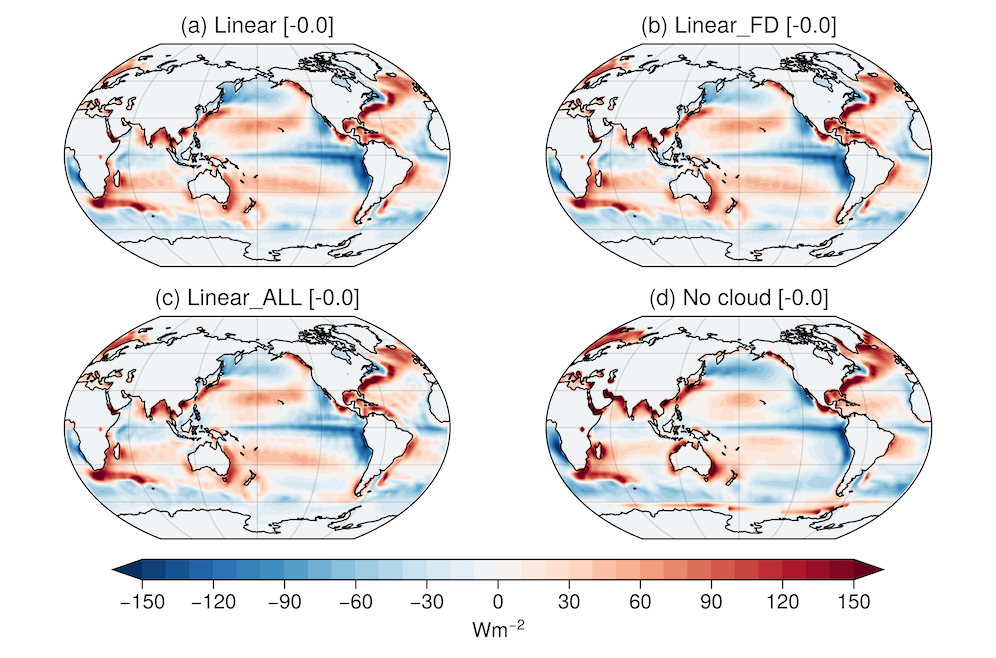
\includegraphics[width=1\linewidth]{{figs/change_of_CRE/Q-flux_cmp}.png}
% 	\caption[Comparison of spatial pattern of ocean heat transport (Q-flux).]{Annual mean Q-flux pattern (in W m$^{-2}$) derived from AMIP fixed-SST experiments with realistic continents and topography. The cloud schemes used are (a) linear, (b) linear\_FD and (c) linear\_ALL as in \tabref{tab:exps} and (d) no cloud scheme.}
% 	\label{fig:Q_flux_cmp}
% \end{figure}

% The AMIP fixed-SST experiments with linear cloud scheme described in \tabref{tab:exps} and a new fixed-SST simulation without clouds are used to derived the Q-flux, and the results are shown in \figref{fig:Q_flux_cmp}. The spatial patterns of Q-flux from different cloud schemes are similar, and have some differences from the simulation without cloud in subtropical and Southern Ocean regions. Q-flux can capture the ocean currents such as the Gulf Stream and cold tongue in the eastern tropical Pacific (\figref{fig:Q_flux_cmp}), and the positive value compensates for too little heating to the slab ocean by the surface flux from the `prescribed-SST’ run compared to the SST climatology. In this case, the Q-flux obtained from the run with the linear cloud scheme only is used in the following simulations. Also, the Q-flux remains the same in the control and perturbed experiments, but it is noted that the SST can change freely in response to different CO$_2$ forcing. 

\subsection{Perturbed parameter ensemble}
 
 \cite{Murphy2004quantification}: a systematic attempt to determine the range of climate changes consistent with these uncertainties, based on a 53-member ensemble of model versions constructed by varying model parameters.
 
 \begin{table}
%\begin{sidewaystable}
	\caption{Design of the perturbed parameter experiments (PPEs). All simulations are run in T42 horizontal resolution.}
	\centering
	\renewcommand{\arraystretch}{1.5}
	\resizebox{\textwidth}{!}{
	\begin{tabular}{c >{\raggedright}m{0.26\linewidth} m{0.6\linewidth}} 
	% control width, alignment for cells
	% https://texblog.org/2017/02/06/proper-tables-with-latex/
		\toprule
	    Experiment & Parameter / Switch & Description \\
		\midrule
		Linear & Default values in \tabref{tab:cld_scheme_summary} & Simulations with Q-flux; Control (1$\times$CO$_2$) and perturbed (4$\times$CO$_2$) experiments \\
		a\_surf & $a_{s}: 42 \rightarrow 20$ & Equivalent to decrease the critical relative humidity at the surface \\
		a\_top & $a_{t}: 13 \rightarrow 10$ & Equivalent to decrease the critical relative humidity at the upper troposphere \\
		Sc\_coeff & $c: -0.1 \rightarrow -0.3$ & The added stratocumulus clouds should decrease \\
		Tmax &  $T_{max}:-5\rightarrow 0~^\circ$C & Increase the temperature threshold of the fraction of liquid cloud (Reff would increase)\\
		Tmin & $T_{min}: -40\rightarrow -20~^\circ$C & Increase the temperature threshold of the fraction of ice cloud\\
		Reff\_ice & $r_{e_ice}:25\rightarrow 50~\mu$m & Increase th default effective radius for ice cloud (Reff would increase)\\
		%rcl\_height &  & In-cloud liquid water mixing ratio is specified as a function of height, rather than as temperature\\
		freezedry & On & Use the freezedry method \\
		Sundqvist & Default values & Change the default cloud fraction scheme from linear to Sundqvist\\
		\bottomrule
	\end{tabular}
	}
	\label{tab:qflux_ppe_exps_summary}
%\end{sidewaystable}
\end{table}

\section{Results}

%\subsection{}

\subsection{COSP evaluation}

\begin{figure}[ht]
    \centering
    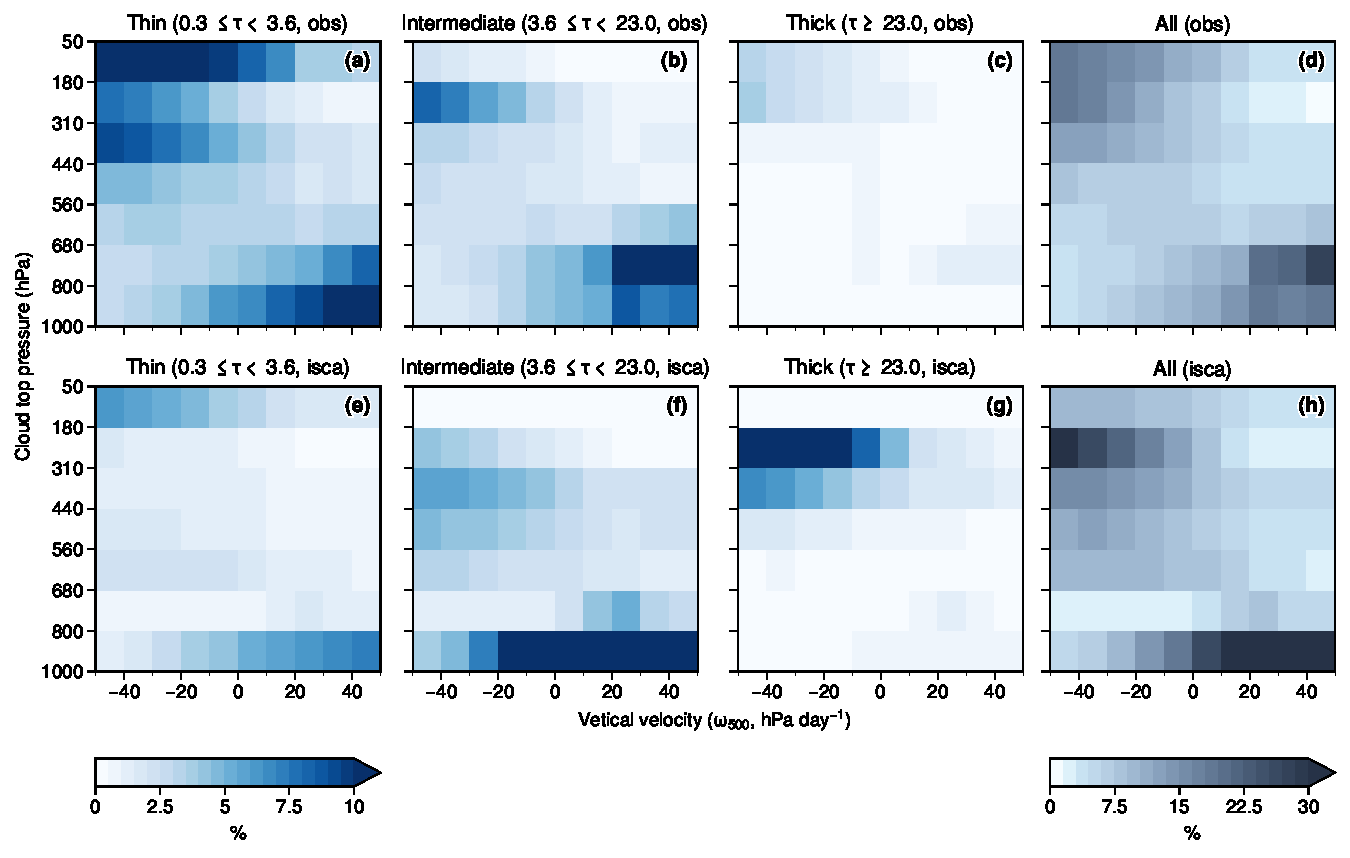
\includegraphics[width=1.0\linewidth]{{figs/change_of_CRE/clisccp_cloud_thickness_category_obs_isca_linear_sc}.pdf}
    \caption{Annual mean cloud frequency from (top row) GCM simulator-oriented ISCCP product (1998-2007) and (bottom row) one Isca simulation, sorted by vertical velocity at 500 hPa ($\omega_{500}$, units: hPa day$^{-1}$) and divided into different cloud thickness categories: (a, e) thin (0.3$\le\tau<$3.6), (b, f) intermediate (3.6$\le\tau<$23), (c, g) thick ($\tau\ge$23), and (d, h) all optical depths. For ISCCP, the $\omega_{500}$ is from ERA-Interim analysis (1998-2007). }
    \label{fig:tropical_clisccp_obs_isca}
\end{figure}

The implementation of COSP provides a new tool to compare Isca simulation results with the observations. Here comparison between Isca simulation and GCM simulator-oriented ISCCP cloud product (covering the period from 1998 to 2007) is shown in \figref{fig:tropical_clisccp_obs_isca}, where the Isca simulation is run with Q-flux with linear and low cloud scheme (shown in \tabref{tab:qflux_ppe_exps_summary}), while the observed cloud amount frequency distribution product is derived from the ISCCP D1 dataset \citep{Rossow1999advances} (available at \url{https://climserv.ipsl.polytechnique.fr/cfmip-obs/data/ISCCP}, last access: June 10, 2021), which is binned into six optical thickness categories, each of which is further divided into seven cloud-top pressure groups. For the Isca simulation with COSP, only ISCCP simulator \citep{Klein1999validation,Webb2001combining} is activated.

\subsection{Comparison of cloud feedback calculation}

\cite{Zelinka2013} has summarized the the diagnostic and methodology used in current studies (see their Table 1). In general, the Gregory method \citep{Gregory2004} that calculates feedback from the slope of $\Delta R$ against $\Delta T_s$ accounts for the rapid adjustments. Here $\Delta R$ is the radiative flux anomaly at the TOA and $\Delta T_s$ is the surface temperature change.  The cloud radiative effect (CRE; i.e. the all-sky minus clear-sky downward radiative flux at TOA) based method is affected by the cloud masking effect, while the cloud radiative kernel method is not affected by this masking effect.

\begin{figure}[ht]
    \centering
    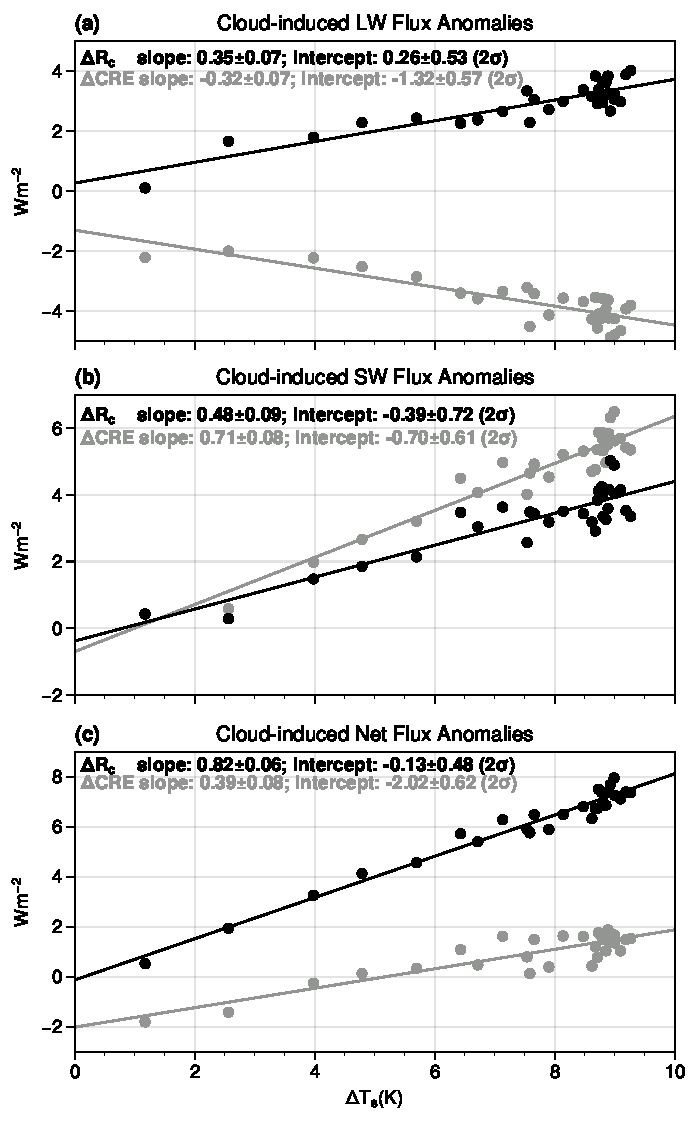
\includegraphics[width=0.6\linewidth]{{figs/change_of_CRE/gregory_plot_all_cld_fbk_v2}.pdf}
    \caption{Global and annual mean anomalies in cloud-induced TOA (a) longwave (LW), (b) shortwave (SW) and (c) net radiative flux against global mean surface temperature change ($\Delta T_s$). The black dots and lines are fluxes derived from cloud radiative kernel method \citep{Zelinka2012computing1, Zelinka2012computing2}, while the gray ones are for the cloud radiative effect (CRE).}
    \label{fig:gregory_plot_for_CRE_and_kernel_flux}
\end{figure}

Here the cloud feedback calculated from these four different methods in Isca simulations are compared and summarized as follows. \figref{fig:gregory_plot_for_CRE_and_kernel_flux} shows the Gregory plot of the global and annual mean anomalies in cloud-induced TOA radiative flux against the change in global mean surface temperature ($\Delta T_s$). These flux anomalies are estimated from CRE and cloud radiative kernel respectively, so they are corresponding to II and IV categories in Table 1 of \cite{Zelinka2013}. It is clear that there is a sign change in the slope of longwave (LW) cloud feedback (\figref{fig:gregory_plot_for_CRE_and_kernel_flux}a), where the slope changed from -0.31 Wm$^{-2}$K$^{-1}$ in category II (CRE+Gregory) to 0.35 Wm$^{-2}$K$^{-1}$ in category IV (kernel+Gregory). The LW forcing term in category II is more negative than that in category IV due to the cloud masking effect. For example, \cite{Andrews2012cloud} found that the instantaneous cloud masking effect for LW CRE is about -0.62 Wm$^{-2}$ in response to doubling CO$_2$ (see their Table 2).


The cloud feedback is also calculated according to categories I and III, and the results are in \tabref{tab:four_methods_cldfbk_results}. Focusing on the second row (the radiative kernel based diagnostic) in \tabref{tab:four_methods_cldfbk_results}, we can find that the cloud feedback parameters from two different methods (categories III and IV in Table 1 of \citealt{Zelinka2013}) are much similar, indicating that neglecting the rapid cloud adjustments has relative small impact on cloud feedback. This is also true for CRE based diagnostic (the first row in \tabref{tab:four_methods_cldfbk_results}). For example, the cloud feedback has relative small changes from category I to category II in Table 1 of \cite{Zelinka2013}. In contrast, comparing to the results from categories I and III (or categories II and IV) suggests that the cloud masking effect do have a large impact on the cloud feedback calculation. For instance, the sign of LW cloud feedback parameter changed from CRE related diagnostic to kernel-derived diagnostic.

\begin{table}[ht]
    %\begin{sidewaystable}
	\caption{Comparison of longwave (LW), shortwave (SW) and net cloud feedbacks estimated from different methods and diagnostics as summarized in Table 1 of \cite{Zelinka2013} (units: Wm$^{-2}$K$^{-1}$).}
	\vspace{0.5em}
	\centering
	\renewcommand{\arraystretch}{1.2}
	\begin{tabular}{>{\centering}m{0.4\linewidth} ccc ccc} 
	    % control width, alignment for cells
	    % https://texblog.org/2017/02/06/proper-tables-with-latex/
		\toprule
		\multirow{2}{*}{Diagnostic} & \multicolumn{3}{c}{$\Delta R/\Delta T_s$} & \multicolumn{3}{c}{\thead{Slope of $\Delta R$ against $\Delta T_s$ \\(Gregory method)}}\\
		\cline{2-4}\cline{5-7}
		 & LW & SW & Net & LW & SW & Net \\
		\midrule
		%CRE anomalies & & & & & & \\
		%Kernel-derived cloud-induced radiation anomalies & & & & & & \\
		CRE anomalies   &  -0.475 &   0.626 &    0.150 &    -0.317 &     0.706 &      0.389 \\  
        Kernel-derived cloud-induced radiation anomalies &   0.365 &   0.440 &    0.805 &     0.346 &     0.479 &      0.825 \\  
        \bottomrule
	\end{tabular}
	\label{tab:four_methods_cldfbk_results}
    %\end{sidewaystable}
\end{table}


\begin{figure}[ht]
    \centering
    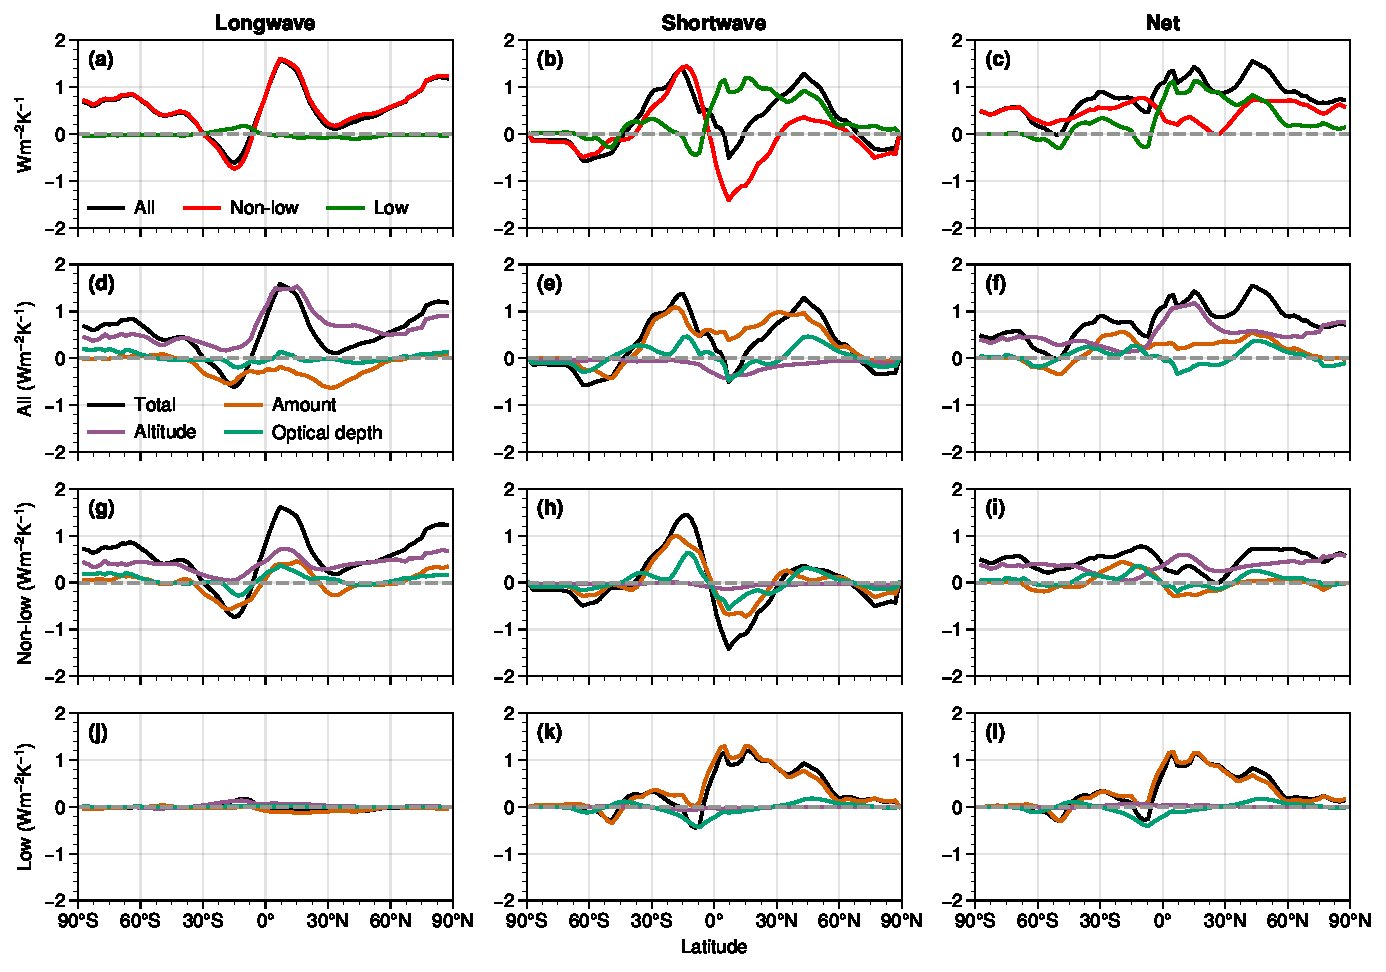
\includegraphics[width=1.0\linewidth]{{figs/change_of_CRE/annual_and_zonal_mean_cld_fbk}.pdf}
    \caption{Zonal and ensemble mean (left column) longwave, (middle column) shortwave, and (right column) net cloud feedbacks from Isca perturbed parameter ensemble. (a-c) Total cloud feedbacks and their separate contributions from non-low (red) and low (green) clouds. Total cloud feedbacks (black) and their amount (orange), altitude (purple), and optical depth (green) components for (d-f) all clouds, (g-i) non-low clouds only, and (j-l) low clouds only.}
    \label{fig:zonal_mean_cld_fbk_ensemble}
\end{figure}

\begin{figure}[ht]
    \centering
    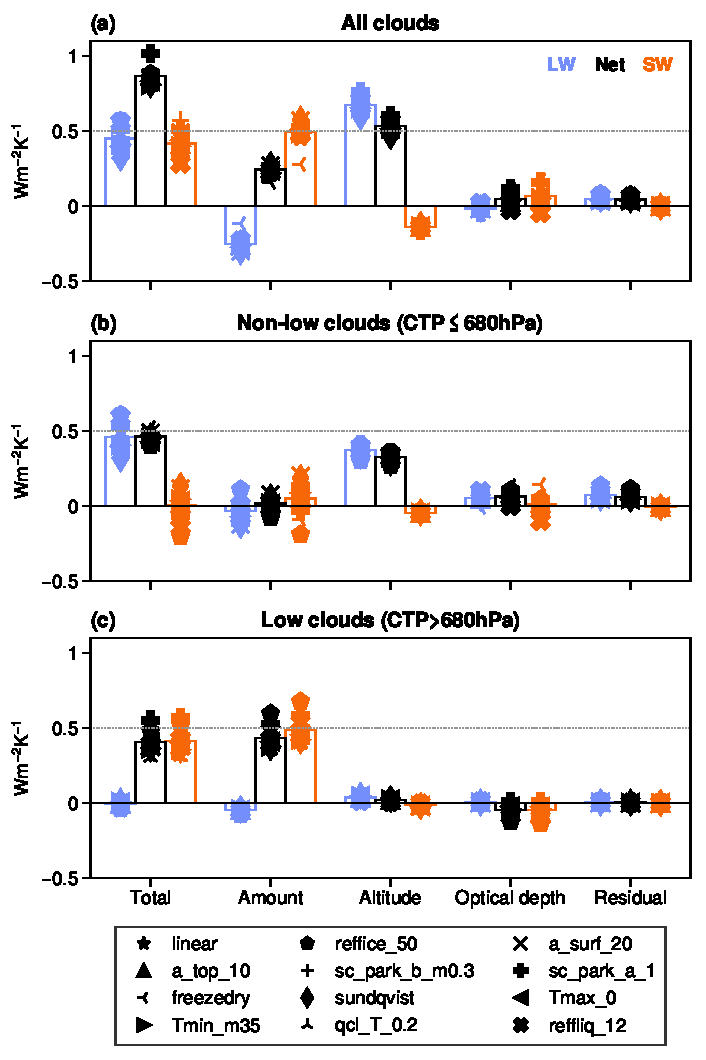
\includegraphics[width=0.8\linewidth]{{figs/change_of_CRE/global_mean_cld_fbk_decomp_scatter}.pdf}
    \caption{Global mean (orange) shortwave (SW), (blue) longwave (LW), and (black) net cloud feedbacks decomposed into amount, altitude, optical depth, and residual components for (a) all clouds, (b) non-low clouds (cloud top pressure, CTP$\le$680 hPa ), and (c) low clouds (CTP > 680hPa). The mean feedbacks of perturbed parameter ensemble are shown as empty bars.}
    \label{fig:global_mean_cld_fbk_scatter}
\end{figure}

\section{Summary and discussion}